% Theoretical background

\chapter{Theoretical background}

\section{Internal flow in circular pipe}

\subsection{Reynolds number}
Reynolds number is one of key points to define fluid properties, predict flow patterns in different fluid situations. It is expressed as a ratio of inertial forces and viscous forces in the fluid. 
\begin{align}
Re & = \frac{Inertial forces}{Viscous forces} = \frac{V_avg D}{\nu} = \frac{\rho V_avg D}{\mu}  \\
V_{avg}  & = \tn{average flow velocity ($m/s$)} \\
D & = \tn{diameter ($m$)} \\
\nu & = \frac{\mu}{\rho} = \tn{kinematic viscosity of fluid ($m^2/s$)} 
\end{align}

The transition flow from laminar to turbulent depends on the degree of disturbance of flow by surface roughness, pipe vibrations and fluctuations in upstream flow (p349) \cite{cengel:book}.In circular pipe, Reynolds number is:
\begin{tabular}{r l}
Re $\leq$ 2300 & laminar flow \\
2300 $\leq$ Re $\leq$ 4000 & transitional flow \\
Re $\geq$ 4000 & turbulent flow
\end{tabular}

\subsection{Laminar flow}

Laminar flow in pipe has Re $\leq$ 2300 which is smooth and highly ordered motion moving in straight line parallel to the surface. The flow is fully developed without any disruption if the pipe is sufficiently long enough (p353) \cite{cengel:book}. There are no cross-currents perpendicular to the direction of flow, nor eddies or swirls of fluids. Laminar flow is a flow establishment indicated  by high momentum diffusion and low momentum convection. Laminar flow is described as a novel flow which usually occurs under highly controlled condition.

\subsection{Turbulent flow}

In our case of investigation, the flow is turbulent as well as most of encountered situations. In daily life, it can be seen under form of surf, storm clouds, fast flowing rivers, etc. Turbulent flow with Re $\geq$ 4000 which is usually chaotic and has rapid fluctuations (p361) \cite{cengel:book}. In turbulent flow, the swirling eddies transport mass, momentum, and energy to other regions of flow much more rapidly than molecular diffusion, greatly enhancing mass, momentum, and heat transfer. Therefore, it usually has higher friction values, heat transfer and mass transfer coefficients. Sometimes, there are unstable vortices in many sizes interacting with each other, which increase friction effects leading to drag effect. The drag effect makes the pump needed more energy to pump fluid through pipe. This  also resonates the pipe or form cavitation that increase energy consumption. While the velocity profile in laminar flow is parabolic, the velocity profile in turbulent flow develops fuller and has sharp drop near pipe wall.  In the pipe, the thin layer next to the wall is called viscous sublayer where viscous effects are major. Next to it is the buffer layer where turbulent effects are getting significant but still affect largely by viscous layer. Above this layer is transition layer, in which the turbulent effects are getting stronger. 

\subsection{Major and Minor Losses}
In a typical piping system, the fluid going through various components like fittings, valves, bends, elbows, reducer, etc in addition to straight section of piping. Major losses are defined by head loss or pressure loss in straight sections and minor losses occurs in the other components of piping. 

\textbf{Pressure loss} is expressed as:

\begin{align}
\Delta P_L & = f \frac{L}{D} \frac{\rho V_{avg}^2 D }{2}   \\
\frac{\rho V_{avg}^2 D }{2}   & = \tn{dynamic pressure} \\
f & = \tn{Darcy- Weisbach friction factor} 
\end{align}

The equivalent expression for pressure loss is well known as equivalent fluid column height or \textbf{head loss}. Head loss represents \textit{the additional height that the fluid needs to be raised by a pump in order to overcome the frictional losses in the pipe} (p356) \cite{cengel:book}.It is obtained by:

\begin{align}
 h_L & =  \frac{\Delta P_L}{\rho g} = f \frac{L}{D} \frac{V_{avg}^2 }{2g}
\end{align}

In another hand, minor losses are usually asserted as loss coefficient K$_{\text{L}}$.  Loss coefficient depends on geometry of component and the Reynolds number. However, Re is usually ignored. It is defined as:

\begin{align}
K_L & =  \frac{h_L}{\nu^2 / (2g)}  \\
h_L  & = \tn{additional irreversible head loss caused by insertion of the component}
\end{align}

When loss coefficient is available, \textbf{minor head loss} for the component can be derived from:

\begin{align}
 h_L & =  K_L \frac{V^2}{2g} = f \frac{L_{equiv}}{D} \frac{V^2 }{2g} \\
 L_{equiv} &= \frac{D}{f} K_L \\
 L_{equiv} &= \tn{equivalent length}
\end{align}

Total head loss in general in piping system is determined from:
\begin{align}
 h_{L, total} & = h_{L, major} + h_{L, minor}
\end{align}

\section{Vortex Flow}
Vortex flow, a major component of turbulent flow, is a region a fluid revolving around an axis line. The fluid flow velocity is strongest close to its axis and reduce in an inverse proportion to the distance of the axis. 
Vortex is best describe by vorticity, a rotation vector of fluid element defined by mathematically by curl of velocity $\vec{V}$. 
There are two types of vortex: irrotational vortex and rotational vortex. Rotational vortices happens the vorticity at a point in flow field is zero and the fluid particle occupying that point is rotating (p156)\cite{cengel:book} . The fluid itself doesn't generate the vortex rotation but external or extra forces which apply on it to keep the motion going indefinitely. Irrotational vortices is also called free vortices. They don't need external forces to maintain the flow. A vortex
evolves fairly quickly toward the irrotational flow pattern, where the flow velocity is inversely proportional to the distance \cite{wiki:web}.

According to Bernoulli's principle (p200) \cite{cengel:book}, the fluid motion in a vortex creates dynamic pressure. This dynamic pressure is lowest in its core region, around the axis, and develops when moving away from it. Firgure \vref{fig:vortexf} presents the vortices after going through Voxer in the test piping system. 

\begin{figure}[h]
  \centering
  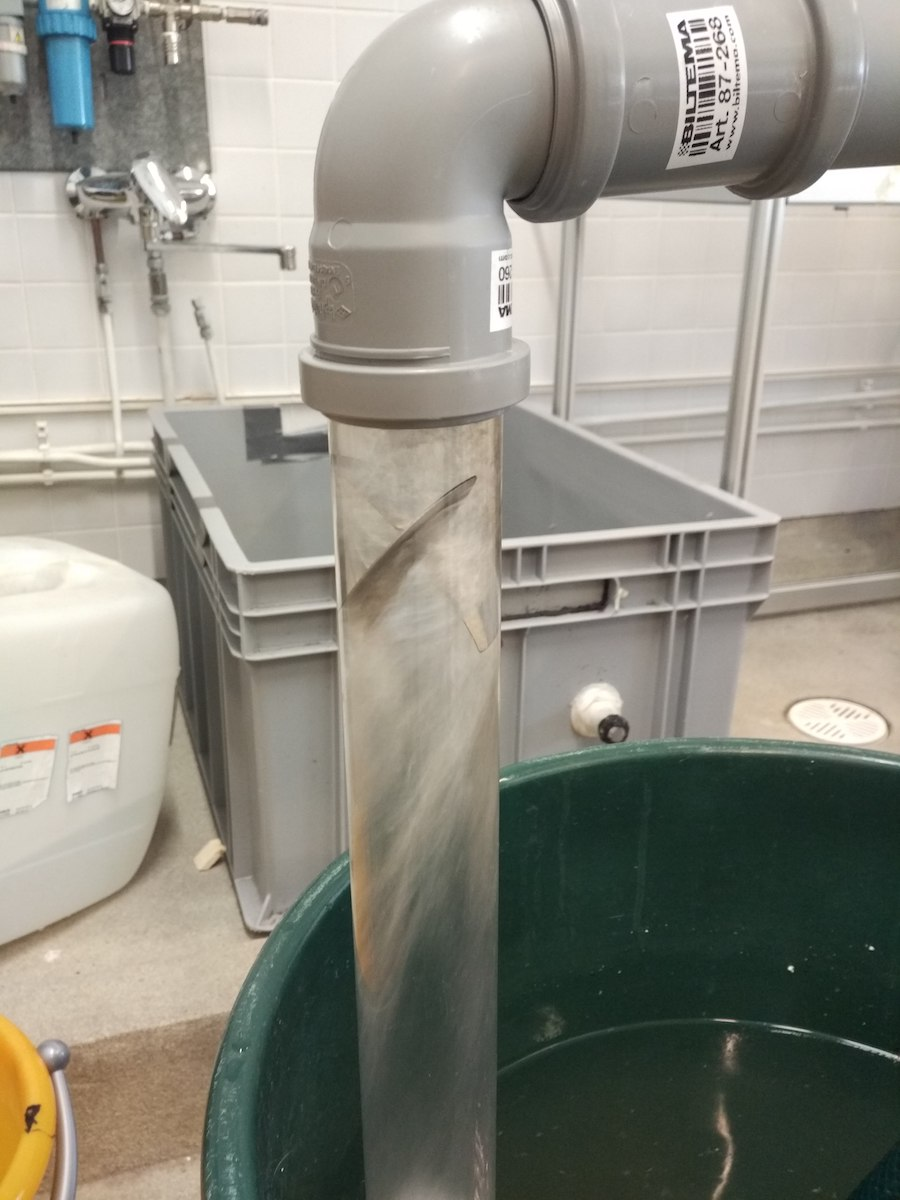
\includegraphics[width=7cm]{vortex}
  \caption{Vortex current after Voxer wing}
  \label{fig:vortexf}
\end{figure}

\section{Motion of flow in 90$^{\circ}$ curve}
From the knowledge in section of minor loss, it is said that these losses would occur when going through curves. In real life condition, the flow motions through curved pipeline are further than complicated being either laminar, transitional or turbulent and through the presence of swirling or pulsations \cite{curve:article}.  When the fluid motion in straight pipe meets the curve, the fluid particle changes their main direction of motion. In the curved conduits, the centrifugal force ($U^{2} / R_{c}$, where U is the velocity and $R_{c}$ is the radius of curvature) induced from the bend will act stronger on the fluid close to the pipe axis than close to the walls. as the higher velocity fluid is next to the pipe axis. This is an adverse pressure gradient generated from the curvature with an increase in pressure, therefore a decrease in velocity close to the convex wall, and the contrary will occur towards the outer side of the pipe. 

\clearpage %force the next chapter to start on a new page. Keep that as the last line of your chapter!
